\documentclass[]{article}
\usepackage{lmodern}
\usepackage{amssymb,amsmath}
\usepackage{ifxetex,ifluatex}
\usepackage{fixltx2e} % provides \textsubscript
\ifnum 0\ifxetex 1\fi\ifluatex 1\fi=0 % if pdftex
  \usepackage[T1]{fontenc}
  \usepackage[utf8]{inputenc}
\else % if luatex or xelatex
  \ifxetex
    \usepackage{mathspec}
  \else
    \usepackage{fontspec}
  \fi
  \defaultfontfeatures{Ligatures=TeX,Scale=MatchLowercase}
\fi
% use upquote if available, for straight quotes in verbatim environments
\IfFileExists{upquote.sty}{\usepackage{upquote}}{}
% use microtype if available
\IfFileExists{microtype.sty}{%
\usepackage{microtype}
\UseMicrotypeSet[protrusion]{basicmath} % disable protrusion for tt fonts
}{}
\usepackage[margin=1in]{geometry}
\usepackage{hyperref}
\hypersetup{unicode=true,
            pdftitle={732A90: Computational Statistics},
            pdfauthor={Sofie Jörgensen, Oriol Garrobé Guilera, David Hrabovszki},
            pdfborder={0 0 0},
            breaklinks=true}
\urlstyle{same}  % don't use monospace font for urls
\usepackage{color}
\usepackage{fancyvrb}
\newcommand{\VerbBar}{|}
\newcommand{\VERB}{\Verb[commandchars=\\\{\}]}
\DefineVerbatimEnvironment{Highlighting}{Verbatim}{commandchars=\\\{\}}
% Add ',fontsize=\small' for more characters per line
\usepackage{framed}
\definecolor{shadecolor}{RGB}{248,248,248}
\newenvironment{Shaded}{\begin{snugshade}}{\end{snugshade}}
\newcommand{\AlertTok}[1]{\textcolor[rgb]{0.94,0.16,0.16}{#1}}
\newcommand{\AnnotationTok}[1]{\textcolor[rgb]{0.56,0.35,0.01}{\textbf{\textit{#1}}}}
\newcommand{\AttributeTok}[1]{\textcolor[rgb]{0.77,0.63,0.00}{#1}}
\newcommand{\BaseNTok}[1]{\textcolor[rgb]{0.00,0.00,0.81}{#1}}
\newcommand{\BuiltInTok}[1]{#1}
\newcommand{\CharTok}[1]{\textcolor[rgb]{0.31,0.60,0.02}{#1}}
\newcommand{\CommentTok}[1]{\textcolor[rgb]{0.56,0.35,0.01}{\textit{#1}}}
\newcommand{\CommentVarTok}[1]{\textcolor[rgb]{0.56,0.35,0.01}{\textbf{\textit{#1}}}}
\newcommand{\ConstantTok}[1]{\textcolor[rgb]{0.00,0.00,0.00}{#1}}
\newcommand{\ControlFlowTok}[1]{\textcolor[rgb]{0.13,0.29,0.53}{\textbf{#1}}}
\newcommand{\DataTypeTok}[1]{\textcolor[rgb]{0.13,0.29,0.53}{#1}}
\newcommand{\DecValTok}[1]{\textcolor[rgb]{0.00,0.00,0.81}{#1}}
\newcommand{\DocumentationTok}[1]{\textcolor[rgb]{0.56,0.35,0.01}{\textbf{\textit{#1}}}}
\newcommand{\ErrorTok}[1]{\textcolor[rgb]{0.64,0.00,0.00}{\textbf{#1}}}
\newcommand{\ExtensionTok}[1]{#1}
\newcommand{\FloatTok}[1]{\textcolor[rgb]{0.00,0.00,0.81}{#1}}
\newcommand{\FunctionTok}[1]{\textcolor[rgb]{0.00,0.00,0.00}{#1}}
\newcommand{\ImportTok}[1]{#1}
\newcommand{\InformationTok}[1]{\textcolor[rgb]{0.56,0.35,0.01}{\textbf{\textit{#1}}}}
\newcommand{\KeywordTok}[1]{\textcolor[rgb]{0.13,0.29,0.53}{\textbf{#1}}}
\newcommand{\NormalTok}[1]{#1}
\newcommand{\OperatorTok}[1]{\textcolor[rgb]{0.81,0.36,0.00}{\textbf{#1}}}
\newcommand{\OtherTok}[1]{\textcolor[rgb]{0.56,0.35,0.01}{#1}}
\newcommand{\PreprocessorTok}[1]{\textcolor[rgb]{0.56,0.35,0.01}{\textit{#1}}}
\newcommand{\RegionMarkerTok}[1]{#1}
\newcommand{\SpecialCharTok}[1]{\textcolor[rgb]{0.00,0.00,0.00}{#1}}
\newcommand{\SpecialStringTok}[1]{\textcolor[rgb]{0.31,0.60,0.02}{#1}}
\newcommand{\StringTok}[1]{\textcolor[rgb]{0.31,0.60,0.02}{#1}}
\newcommand{\VariableTok}[1]{\textcolor[rgb]{0.00,0.00,0.00}{#1}}
\newcommand{\VerbatimStringTok}[1]{\textcolor[rgb]{0.31,0.60,0.02}{#1}}
\newcommand{\WarningTok}[1]{\textcolor[rgb]{0.56,0.35,0.01}{\textbf{\textit{#1}}}}
\usepackage{graphicx,grffile}
\makeatletter
\def\maxwidth{\ifdim\Gin@nat@width>\linewidth\linewidth\else\Gin@nat@width\fi}
\def\maxheight{\ifdim\Gin@nat@height>\textheight\textheight\else\Gin@nat@height\fi}
\makeatother
% Scale images if necessary, so that they will not overflow the page
% margins by default, and it is still possible to overwrite the defaults
% using explicit options in \includegraphics[width, height, ...]{}
\setkeys{Gin}{width=\maxwidth,height=\maxheight,keepaspectratio}
\IfFileExists{parskip.sty}{%
\usepackage{parskip}
}{% else
\setlength{\parindent}{0pt}
\setlength{\parskip}{6pt plus 2pt minus 1pt}
}
\setlength{\emergencystretch}{3em}  % prevent overfull lines
\providecommand{\tightlist}{%
  \setlength{\itemsep}{0pt}\setlength{\parskip}{0pt}}
\setcounter{secnumdepth}{0}
% Redefines (sub)paragraphs to behave more like sections
\ifx\paragraph\undefined\else
\let\oldparagraph\paragraph
\renewcommand{\paragraph}[1]{\oldparagraph{#1}\mbox{}}
\fi
\ifx\subparagraph\undefined\else
\let\oldsubparagraph\subparagraph
\renewcommand{\subparagraph}[1]{\oldsubparagraph{#1}\mbox{}}
\fi

%%% Use protect on footnotes to avoid problems with footnotes in titles
\let\rmarkdownfootnote\footnote%
\def\footnote{\protect\rmarkdownfootnote}

%%% Change title format to be more compact
\usepackage{titling}

% Create subtitle command for use in maketitle
\providecommand{\subtitle}[1]{
  \posttitle{
    \begin{center}\large#1\end{center}
    }
}

\setlength{\droptitle}{-2em}

  \title{732A90: Computational Statistics}
    \pretitle{\vspace{\droptitle}\centering\huge}
  \posttitle{\par}
  \subtitle{Computer lab4 - Group11}
  \author{Sofie Jörgensen, Oriol Garrobé Guilera, David Hrabovszki}
    \preauthor{\centering\large\emph}
  \postauthor{\par}
      \predate{\centering\large\emph}
  \postdate{\par}
    \date{19 February 2020}

\usepackage{float}
\let\origfigure\figure
\let\endorigfigure\endfigure
\renewenvironment{figure}[1][2] {
    \expandafter\origfigure\expandafter[H]
} {
    \endorigfigure
}

\begin{document}
\maketitle

\hypertarget{question-1-computations-with-metropolis-hastings}{%
\section{Question 1: Computations with
Metropolis-Hastings}\label{question-1-computations-with-metropolis-hastings}}

In this question we define the density function \(f(x)\) as

\[f(x)\propto x^5e^{-x}, \quad x>0.\] This density function is known up
to some constant of proportionality, which is 120.

\hypertarget{section}{%
\subsubsection{1.}\label{section}}

In the first step we use the Metropolis-Hastings algorithm to generate
samples from the posterior distribution \(f(x)\) by using the log-normal
\(LN(X_t,1)\) as the proposal distribution. We take 1 as a starting
point, because we expect this value to be within the range of possible
values of the distribution defined above.

The time series plot of the obtained chain of samples can be observed in
Figure \ref{fig:lognormal}. The plot does not show that the chain
converges, because it often takes the same value for many iterations and
then jumps to a very different one. This implies that the sample is not
close to the posterior. There does not seem to be a burn-in period,
because samples from many iterations are close to the starting point
(which was 1 in this case).

\begin{figure}[h]

{\centering 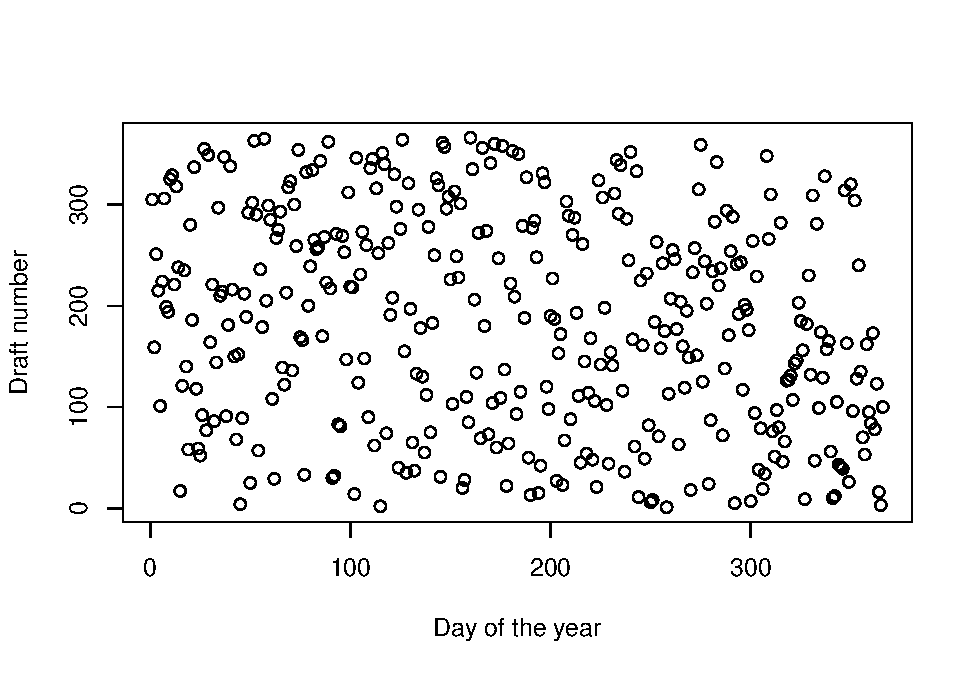
\includegraphics[width=0.8\linewidth]{Lab4_Group11_files/figure-latex/unnamed-chunk-3-1} 

}

\caption{\label{fig:lognormal} Metropolis-Hastings sampler with log-normal proposal}\label{fig:unnamed-chunk-3}
\end{figure}

\begin{figure}[h]

{\centering \includegraphics[width=0.8\linewidth]{Lab4_Group11_files/figure-latex/unnamed-chunk-4-1} 

}

\caption{\label{fig:lognormal_hist} Histogram of generated samples with log-normal proposal (MH sampler)}\label{fig:unnamed-chunk-4}
\end{figure}

\hypertarget{section-1}{%
\subsubsection{2.}\label{section-1}}

Now we perform Step 1 using the chi-square distribution
\(\chi^2(\lfloor X_t+1\rfloor)\) as the proposal distribution, where
\(\lfloor x\rfloor\) is the \texttt{floor()} function.

The time series plot is shown in Figure \ref{fig:chisquare}, and it can
be seen that the chain converges much more than in the previous case.
Again there does not seem to be a burn-in period, the starting value of
1 seems to be a probable value of the distribution, so we do not discard
any samples from the beginning of the chain.

\begin{figure}[h]

{\centering 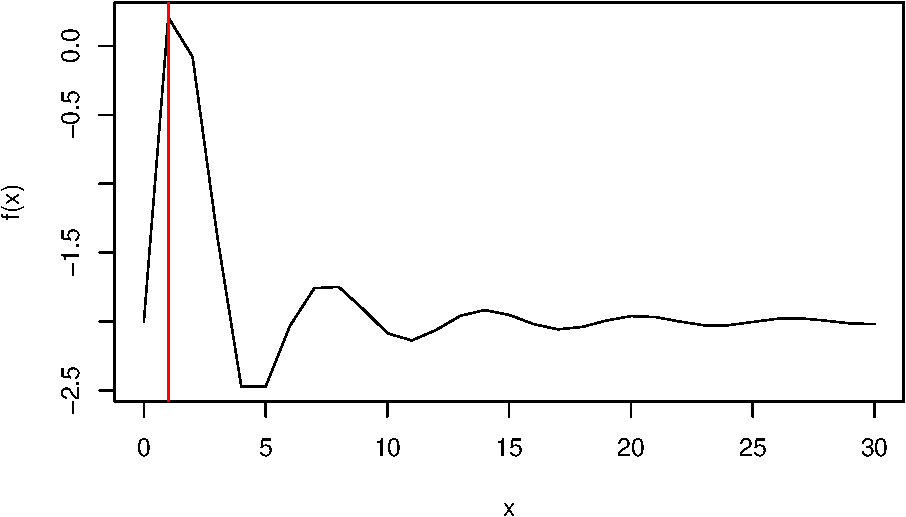
\includegraphics[width=0.8\linewidth]{Lab4_Group11_files/figure-latex/unnamed-chunk-6-1} 

}

\caption{\label{fig:chisquare} Metropolis-Hastings sampler with chi-square proposal}\label{fig:unnamed-chunk-6}
\end{figure}

\begin{figure}[h]

{\centering \includegraphics[width=0.8\linewidth]{Lab4_Group11_files/figure-latex/unnamed-chunk-7-1} 

}

\caption{\label{fig:chisquare_hist} Histogram of generated samples with Chi-square proposal (MH sampler)}\label{fig:unnamed-chunk-7}
\end{figure}

\hypertarget{section-2}{%
\subsubsection{3.}\label{section-2}}

We recognise that the probability distribution function \(f(x)\) belongs
to a certain gamma distribution, therefore we know that \(f(x)\) must
have a positive skew. This attribute is also true for the distribution
of samples from Step 2 (Figure \ref{fig:chisquare_hist}), but untrue for
the distribution of samples from Step 1 (Figure
\ref{fig:lognormal_hist}). Also, the chain with the log-normal proposal
does not converge, but the chain with the Chi-square proposal does, so
we conclude that the samples generated from Step 2 are a better
approximation of samples from the posterior distribution.

\hypertarget{section-3}{%
\subsubsection{4.}\label{section-3}}

Now we generate 10 MCMC sequences using the sample generator from Step
2, and analyze their convergence using the Gelman-Rubin method. The
starting points for the 10 sequences are 1,2,\ldots{},10.

The output of the Gelman-Rubin's convergence diagnostic for 1000
iterations gives the potential scale reduction factors with the
corresponding point estimate and the upper confidence limit. The
potential scale reduction factor is based on the comparison of
within-chain and between-chain variances. For 1000 iterations, its point
estimate is 1.01 and its upper confidence limit is 1.02, which is very
close to 1. So according to this diagnostics, approximate convergence
has been achieved at 1000 iterations. Even for only 100 iterations, both
the point estimate and the upper limit are under 1.1.

\hypertarget{section-4}{%
\subsubsection{5.}\label{section-4}}

In this step we estimate

\[\int\limits_{0}^{\infty}xf(x)dx\] using the samples generated from
Steps 1 and 2.

Based on the slides from Lecture 4 we can use MCMC samples from
\(p(\theta|D)\) to obtain a point estimator by calculating the sample
average:
\[\theta^* = \int\theta p(\theta|D) \approx \frac{1}{n} \sum\limits_{i=1}^{n}\theta_i\]

The sample average of the chain generated in Step 1 is \textbf{2.95} and
in Step 2 is \textbf{5.63}.

If we do not set the seed before the sample generation, then we get
highly variable averages from Step 1, but from Step 2 it is almost
always between 5.5 and 6.5.

\hypertarget{section-5}{%
\subsubsection{6.}\label{section-5}}

According to Definition 4.5 in Mathematical Statistics with Applications
by Wackerly et al., the integral in Step 5 is equal to the expected
value of random variable X, where X can take values between 0 and
\(\infty\).

The generated distribution with probability density function \(f(x)\) is
a gamma distribution, so we can express \(f(x)\) in its general form as
\[f(x) = \Bigg{[}\frac{1}{\Gamma(\alpha)\beta^\alpha}\Bigg{]}x^{\alpha-1}e^{-x/\beta},\]

where \(0<x<\infty\). Thus \(E(X) = \alpha\beta\). In our case
\(\alpha = 6, \beta=1\), so \(E(X) = 6\).

This is the actual value of the integral in Step 5, so we conclude that
our estimation using the samples generated in Step 2 with a Chi-square
proposal distribution seems accurate, whereas the estimation from the
samples of Step 1 with the log-normal proposal does not seem accurate at
all.

\begin{center}\rule{0.5\linewidth}{\linethickness}\end{center}

\hypertarget{question-2-gibbs-sampling}{%
\section{Question 2: Gibbs sampling}\label{question-2-gibbs-sampling}}

\hypertarget{section-6}{%
\subsubsection{1.}\label{section-6}}

The aim of this task is to restore the expected concentration values,
given the data \texttt{chemical.RData}. We import the data into R,
containing the concentration of a certain chemical in a water sample,
having the following variables:

\begin{itemize}
\tightlist
\item
  \texttt{X}: day of the measurment,
\item
  \texttt{Y}: measured concentration of the chemical.
\end{itemize}

The code can be found in the Appendix.

Figure \ref{fig:chemical} shows the the dependence of \texttt{Y} on
\texttt{X}, where a linear relationship between \texttt{Y} and
\texttt{X} can be observed. Therefore a linear regression with normally
distributed residuals seems like a good approach.

\begin{figure}[h]

{\centering \includegraphics[width=0.8\linewidth]{Lab4_Group11_files/figure-latex/unnamed-chunk-11-1} 

}

\caption{\label{fig:chemical} Dependendence of measured concentration of the chemical on day of the measurment}\label{fig:unnamed-chunk-11}
\end{figure}

\hypertarget{section-7}{%
\subsubsection{2.}\label{section-7}}

Using the random-walk Bayesian model
\(Y_{i} \sim N(\mu_{i}, \sigma^2=0.2)\) for \(i=1,...,n\), with the
prior \(p(\mu_1)=1\), \(p(\mu_{i+1}|\mu_i)=N(\mu_i,\sigma^2=0.2)\), for
\(i=1,...,{n-1}\). We denote the the number of observations with \(n\)
and we consider \(\vec{\mu}=(\mu_{1},...,\mu_{n})\) as unknown
parameters.

Given this information we are able to compute the likelihood
\(p(\vec{Y}|\vec{\mu})\). Under the assumption that \(Y_i\) are iid, the
likelihood is given by

\begin{eqnarray*}
p(\vec{Y}|\vec{\mu}) &=& \prod_{i=1}^{n}f(Y_{i}|\mu_{i},\sigma^2) \\
                     &=& \prod_{i=1}^{n}\frac{1}{\sigma\sqrt{2\pi}} \ \text{exp}\left[-\frac{(Y_{i}-\mu_{i})^2}{2\sigma^{2}}\right]\\
                     &=& \left(\frac{1}{\sigma\sqrt{2\pi}}\right)^n \text{exp}\left[-\frac{\sum_{i=1}^{n}(Y_{i}-\mu_{i})^2}{2\sigma^{2}}\right].\\
\end{eqnarray*}

Further, we will compute the prior by using the chain rule
\(p(\vec{\mu})=p(\mu_{1})p(\mu_{2}|\mu_{1})...p(\mu_{n}|\mu_{n-1})\).
Then the prior is given by \begin{eqnarray*}
p(\vec{\mu}) &=& p(\mu_1)\prod_{i=1}^{n-1}p(\mu_{i+1}|\mu_{i}) \\
             &=& \prod_{i=2}^{n}\frac{1}{\sigma\sqrt{2\pi}} \ \text{exp}\left[-\frac{(\mu_{i}-\mu_{i-1})^2}{2\sigma^{2}}\right]\\
             &=& \left(\frac{1}{\sigma\sqrt{2\pi}}\right)^n \text{exp} \left[-\frac{\sum_{i=2}^{n}(\mu_{i}-\mu_{i-1})^2}{2\sigma^{2}}\right]. \\
\end{eqnarray*}

\hypertarget{section-8}{%
\subsubsection{3.}\label{section-8}}

In order to get the posterior, up to a constant proportionality, we use
the Bayes' Theorem. Therefore,

\begin{eqnarray*}
p(\vec{\mu}|\vec{Y}) &\propto& p(\vec{Y}|\vec{\mu})p(\vec{\mu})\\
                     &\propto& \left(\frac{1}{\sigma\sqrt{2\pi}}\right)^n \text{exp}\left[-\frac{\sum_{i=1}^{n}(Y_{i}-\mu_{i})^2}{2\sigma^{2}}\right] \left(\frac{1}{\sigma\sqrt{2\pi}}\right)^n \text{exp}\left[-\frac{\sum_{i=2}^{n}(\mu_{i}-\mu_{i-1})^2}{2\sigma^{2}}\right]\\
                     &\propto& \text{exp}\left[-\frac{\sum_{i=1}^{n}(Y_{i}-\mu_{i})^2}{2\sigma^{2}}\right] \text{exp}\left[-\frac{\sum_{i=2}^{n}(\mu_{i}-\mu_{i-1})^2}{2\sigma^{2}}\right]\\
                     &\propto& \text{exp}\left[-\frac{\sum_{i=1}^{n}(Y_{i}-\mu_{i})^2 + \sum_{i=2}^{n}(\mu_{i}-\mu_{i-1})^2}{2\sigma^{2}}\right].
\end{eqnarray*}

And finally, once we have the posterior, we can compute the the
probability distribution \(p(\mu_{i}|\vec{\mu}_{i},\vec{Y})\), where
\(\vec\mu_{-i}\) is a vector containing all \(\mu\) values except for
\(\mu_{i}\). We also know that we can discard all the elements that do
not contain \(\vec\mu_{i}\), as we are looking for a posterior up to a
constant proportionality. Given Hint A, we will consider separate
formulas for \(p(\mu_{1}|\vec{\mu}_{1},\vec{Y})\) and for
\(p(\mu_{n}|\vec{\mu}_{n},\vec{Y})\). By using Hint B, we obtain

\[p(\mu_{1}|\vec{\mu}_{-1},\vec{Y}) \propto \text{exp}\left[-\frac{\left(\mu_{1}-(Y_{1}+\mu_{2})/2\right)^{2}}{\sigma^{2}}\right], \quad \text{for }i=1,\]

and

\[p(\mu_{n}|\vec{\mu}_{-1},\vec{Y}) \propto \text{exp}\left[-\frac{\left(\mu_{n}-(Y_{n}+\mu_{n-1})/2\right)^{2}}{\sigma^{2}}\right], \quad \text{for }i=n.\]

By using Hint C, we get to the result

\[p(\mu_{i}|\vec{\mu}_{-i},\vec{Y}) \propto \text{exp}\left[-\frac{\left(\mu_{i}-(Y_{i}+\mu_{i-1}+\mu_{i+1})/3\right)^{2}}{2\sigma^{2}/3}\right], \quad \text{for } i=2,...,n-1.\]

\hypertarget{section-9}{%
\subsubsection{4.}\label{section-9}}

We implement the Gibbs samples using the distributions found and initial
value \(\vec\mu^{0}=(0,...,0)\). This code snippet (see Appendix)
computes \(n\) values of \(\vec\mu\) and computes the expected value of
\(\vec\mu\) using a Monte Carlo approach. In this particular case
\(n=1000\).

The expected value of \(\vec\mu\) is:

In \ref{fig:gibbs} there is a plot of the dependence of \texttt{Y} on
\texttt{X} and the comparison with the expected values of mu.

\begin{figure}[h]

{\centering \includegraphics[width=0.8\linewidth]{Lab4_Group11_files/figure-latex/unnamed-chunk-13-1} 

}

\caption{\label{fig:gibbs} Comparison between Y and expected value of mu}\label{fig:unnamed-chunk-13}
\end{figure}

The result is considered as positive as observing the plot it is
possible to see that the expected values of \(\mu\) follow the same
pattern that \texttt{Y} in terms of dependence on \texttt{X}. Also, the
expected values seem to have removed the noise produced by the accuracy
of the instrumentat used to measure, as the expected values of \(mu\)
are less spread than those of \texttt{Y}.

\hypertarget{section-10}{%
\subsubsection{5.}\label{section-10}}

\begin{figure}[h]

{\centering \includegraphics[width=0.8\linewidth]{Lab4_Group11_files/figure-latex/unnamed-chunk-14-1} 

}

\caption{\label{fig:burn_in} Burn in period and convergence}\label{fig:unnamed-chunk-14}
\end{figure}

In order to verify that the MCMC explores the parameter space
efficiently, we want to assure that the chain does not stay in the same
state for too long or has too many consecutive steps in one direction.
In this case, the traceplot behaves accordingly.

Burning in is a method that erases iterations at the beginning of a
Markov Chain Monte Carlo (MCMC) run, it is a way to select a better
starting point that just one by random. It can be seen from the plot
that there is a burn in period of 1 iteration, after that one the value
of mu moves between 1.25 and 1.75.

\hypertarget{section-11}{%
\subsection{\texorpdfstring{\pagebreak}{}}\label{section-11}}

\hypertarget{appendix}{%
\section{Appendix}\label{appendix}}

\begin{Shaded}
\begin{Highlighting}[]
\NormalTok{knitr}\OperatorTok{::}\NormalTok{opts_chunk}\OperatorTok{$}\KeywordTok{set}\NormalTok{(}\DataTypeTok{echo =} \OtherTok{FALSE}\NormalTok{)}
\CommentTok{# R version}
\KeywordTok{RNGversion}\NormalTok{(}\StringTok{'3.5.1'}\NormalTok{)}
\CommentTok{#libraries}
\KeywordTok{library}\NormalTok{(coda)}

\CommentTok{# 1.1.}
\NormalTok{posterior <-}\StringTok{ }\ControlFlowTok{function}\NormalTok{(x)\{}
\NormalTok{  x}\OperatorTok{^}\DecValTok{5} \OperatorTok{*}\StringTok{ }\KeywordTok{exp}\NormalTok{(}\OperatorTok{-}\NormalTok{x)}
\NormalTok{\}}

\CommentTok{# Seed}
\KeywordTok{set.seed}\NormalTok{(}\DecValTok{1234567890}\NormalTok{)}

\NormalTok{posterior_sampler_ln <-}\StringTok{ }\ControlFlowTok{function}\NormalTok{(}\DataTypeTok{tmax=}\DecValTok{1000}\NormalTok{, }\DataTypeTok{starting_point =} \DecValTok{1}\NormalTok{) \{}
\NormalTok{  X=}\KeywordTok{rep}\NormalTok{(starting_point,tmax)}
  \ControlFlowTok{for}\NormalTok{ (t }\ControlFlowTok{in} \DecValTok{1}\OperatorTok{:}\NormalTok{tmax) \{}
\NormalTok{    Y =}\StringTok{ }\KeywordTok{rlnorm}\NormalTok{(}\DecValTok{1}\NormalTok{,}\DataTypeTok{meanlog =}\NormalTok{ X[t],}\DataTypeTok{sdlog =} \DecValTok{1}\NormalTok{)}
\NormalTok{    U =}\StringTok{ }\KeywordTok{runif}\NormalTok{(}\DecValTok{1}\NormalTok{,}\DataTypeTok{min =} \DecValTok{0}\NormalTok{, }\DataTypeTok{max =} \DecValTok{1}\NormalTok{)}
\NormalTok{    alpha =}\StringTok{ }\KeywordTok{min}\NormalTok{(}\DecValTok{1}\NormalTok{,}
\NormalTok{                (}\KeywordTok{posterior}\NormalTok{(Y) }\OperatorTok{*}\StringTok{ }\KeywordTok{dlnorm}\NormalTok{(X[t],}\DataTypeTok{meanlog =}\NormalTok{ Y, }\DataTypeTok{sdlog =} \DecValTok{1}\NormalTok{)) }\OperatorTok{/}
\StringTok{                }\NormalTok{(}\KeywordTok{posterior}\NormalTok{(X[t]) }\OperatorTok{*}\StringTok{ }\KeywordTok{dlnorm}\NormalTok{(Y, }\DataTypeTok{meanlog =}\NormalTok{ X[t], }\DataTypeTok{sdlog =} \DecValTok{1}\NormalTok{)))}
    \ControlFlowTok{if}\NormalTok{ (U }\OperatorTok{<}\StringTok{ }\NormalTok{alpha) \{}
\NormalTok{      X[t}\OperatorTok{+}\DecValTok{1}\NormalTok{] =}\StringTok{ }\NormalTok{Y}
\NormalTok{    \} }\ControlFlowTok{else}\NormalTok{ \{}
\NormalTok{      X[t}\OperatorTok{+}\DecValTok{1}\NormalTok{] =}\StringTok{ }\NormalTok{X[t]}
\NormalTok{    \}}
\NormalTok{    t =}\StringTok{ }\NormalTok{t}\OperatorTok{+}\DecValTok{1}
\NormalTok{  \}}
  \KeywordTok{return}\NormalTok{(X)}
\NormalTok{\}}
\NormalTok{tmax=}\DecValTok{1000}
\CommentTok{# Seed}
\KeywordTok{set.seed}\NormalTok{(}\DecValTok{1234567890}\NormalTok{)}
\NormalTok{ln_sample =}\StringTok{ }\KeywordTok{posterior_sampler_ln}\NormalTok{(}\DataTypeTok{tmax =}\NormalTok{ tmax, }\DataTypeTok{starting_point =} \DecValTok{1}\NormalTok{)}
\KeywordTok{plot}\NormalTok{(}\DecValTok{1}\OperatorTok{:}\NormalTok{(tmax}\OperatorTok{+}\DecValTok{1}\NormalTok{),ln_sample, }\DataTypeTok{type =}\StringTok{'l'}\NormalTok{, }\DataTypeTok{xlab =} \StringTok{"time"}\NormalTok{, }\DataTypeTok{ylab =} \StringTok{"X"}\NormalTok{)}

\KeywordTok{hist}\NormalTok{(ln_sample, }\DataTypeTok{breaks =} \DecValTok{20}\NormalTok{, }\DataTypeTok{main =} \StringTok{""}\NormalTok{, }\DataTypeTok{xlab =} \StringTok{"X"}\NormalTok{)}

\CommentTok{# 1.2}
\CommentTok{#Set seed}
\KeywordTok{set.seed}\NormalTok{(}\DecValTok{1234567890}\NormalTok{)}

\NormalTok{posterior_sampler_chisq <-}\StringTok{ }\ControlFlowTok{function}\NormalTok{(}\DataTypeTok{tmax=}\DecValTok{1000}\NormalTok{, }\DataTypeTok{starting_point =} \DecValTok{1}\NormalTok{) \{}
\NormalTok{  X=}\KeywordTok{rep}\NormalTok{(starting_point,tmax)}
  \ControlFlowTok{for}\NormalTok{ (t }\ControlFlowTok{in} \DecValTok{1}\OperatorTok{:}\NormalTok{tmax) \{}
\NormalTok{    Y =}\StringTok{ }\KeywordTok{rchisq}\NormalTok{(}\DecValTok{1}\NormalTok{,}\DataTypeTok{df =} \KeywordTok{floor}\NormalTok{(X[t]}\OperatorTok{+}\DecValTok{1}\NormalTok{))}
\NormalTok{    U =}\StringTok{ }\KeywordTok{runif}\NormalTok{(}\DecValTok{1}\NormalTok{,}\DataTypeTok{min =} \DecValTok{0}\NormalTok{, }\DataTypeTok{max =} \DecValTok{1}\NormalTok{)}
\NormalTok{    alpha =}\StringTok{ }\KeywordTok{min}\NormalTok{(}\DecValTok{1}\NormalTok{,}
\NormalTok{                (}\KeywordTok{posterior}\NormalTok{(Y) }\OperatorTok{*}\StringTok{ }\KeywordTok{dchisq}\NormalTok{(X[t],}\DataTypeTok{df =} \KeywordTok{floor}\NormalTok{(Y}\OperatorTok{+}\DecValTok{1}\NormalTok{))) }\OperatorTok{/}
\StringTok{                }\NormalTok{(}\KeywordTok{posterior}\NormalTok{(X[t]) }\OperatorTok{*}\StringTok{ }\KeywordTok{dchisq}\NormalTok{(Y, }\DataTypeTok{df =} \KeywordTok{floor}\NormalTok{(X[t]}\OperatorTok{+}\DecValTok{1}\NormalTok{))))}
    \ControlFlowTok{if}\NormalTok{ (U }\OperatorTok{<}\StringTok{ }\NormalTok{alpha) \{}
\NormalTok{      X[t}\OperatorTok{+}\DecValTok{1}\NormalTok{] =}\StringTok{ }\NormalTok{Y}
\NormalTok{    \} }\ControlFlowTok{else}\NormalTok{ \{}
\NormalTok{      X[t}\OperatorTok{+}\DecValTok{1}\NormalTok{] =}\StringTok{ }\NormalTok{X[t]}
\NormalTok{    \}}
\NormalTok{    t =}\StringTok{ }\NormalTok{t}\OperatorTok{+}\DecValTok{1}
\NormalTok{  \}}
  \KeywordTok{return}\NormalTok{(X)}
\NormalTok{\}}
\NormalTok{tmax=}\DecValTok{1000}
\CommentTok{# Seed}
\KeywordTok{set.seed}\NormalTok{(}\DecValTok{1234567890}\NormalTok{)}
\NormalTok{chi_sample =}\StringTok{ }\KeywordTok{posterior_sampler_chisq}\NormalTok{(}\DataTypeTok{tmax =}\NormalTok{ tmax, }\DataTypeTok{starting_point =} \DecValTok{1}\NormalTok{)}
\KeywordTok{plot}\NormalTok{(}\DecValTok{1}\OperatorTok{:}\NormalTok{(tmax}\OperatorTok{+}\DecValTok{1}\NormalTok{), chi_sample, }\DataTypeTok{type =} \StringTok{'l'}\NormalTok{, }\DataTypeTok{xlab =} \StringTok{"time"}\NormalTok{, }\DataTypeTok{ylab =} \StringTok{"X"}\NormalTok{)}
\KeywordTok{hist}\NormalTok{(chi_sample, }\DataTypeTok{breaks =} \DecValTok{20}\NormalTok{, }\DataTypeTok{main =} \StringTok{""}\NormalTok{, }\DataTypeTok{xlab =} \StringTok{"X"}\NormalTok{)}

\CommentTok{#1.4}
\NormalTok{starting_points =}\StringTok{ }\KeywordTok{seq}\NormalTok{(}\DecValTok{1}\NormalTok{,}\DecValTok{10}\NormalTok{)}
\NormalTok{MCMC_seqs =}\StringTok{ }\KeywordTok{mcmc.list}\NormalTok{()}
\NormalTok{tmax=}\DecValTok{1000}
\CommentTok{# Seed}
\KeywordTok{set.seed}\NormalTok{(}\DecValTok{1234567890}\NormalTok{)}
\ControlFlowTok{for}\NormalTok{ (k }\ControlFlowTok{in}\NormalTok{ starting_points) \{}
\NormalTok{  MCMC_seqs[[k]] =}\StringTok{ }\KeywordTok{as.mcmc}\NormalTok{(}\KeywordTok{posterior_sampler_chisq}\NormalTok{(}\DataTypeTok{tmax =}\NormalTok{ tmax, }\DataTypeTok{starting_point =}\NormalTok{ k))}
\NormalTok{\}}

\KeywordTok{print}\NormalTok{(}\KeywordTok{gelman.diag}\NormalTok{(MCMC_seqs))}

\CommentTok{# 1.5}
\CommentTok{# Seed}
\KeywordTok{set.seed}\NormalTok{(}\DecValTok{1234567890}\NormalTok{)}
\CommentTok{#using Step1}
\CommentTok{#mean(ln_sample) #large variance; 2.949404}

\CommentTok{#using Step2}
\CommentTok{#mean(chi_sample) #small variance; 5.636084}


\CommentTok{############################## Question 2: Gibbs sampling ###############################}

\KeywordTok{load}\NormalTok{(}\DataTypeTok{file =} \StringTok{"chemical.RData"}\NormalTok{) }
\CommentTok{# 2.1}

\KeywordTok{plot}\NormalTok{(X,Y, }\DataTypeTok{xlab =} \StringTok{"Day of the measurment"}
\NormalTok{     , }\DataTypeTok{ylab =} \StringTok{"Measured concentration of the chemical"}\NormalTok{, }\DataTypeTok{col =} \StringTok{"grey"}\NormalTok{, }\DataTypeTok{pch =} \DecValTok{16}\NormalTok{)}
\CommentTok{# 2.4}

\NormalTok{gibbs_sampler <-}\StringTok{ }\ControlFlowTok{function}\NormalTok{(Tmax) \{}
\NormalTok{  d <-}\StringTok{ }\KeywordTok{length}\NormalTok{(Y)}
\NormalTok{  sigma <-}\StringTok{ }\FloatTok{0.2}
\NormalTok{  mu <-}\StringTok{ }\KeywordTok{matrix}\NormalTok{(}\DecValTok{0}\NormalTok{, }\DataTypeTok{nrow =}\NormalTok{ Tmax, }\DataTypeTok{ncol =}\NormalTok{ d)}
\NormalTok{  t <-}\StringTok{ }\DecValTok{1}
  \ControlFlowTok{while}\NormalTok{ (t}\OperatorTok{<}\NormalTok{Tmax) \{}
    \ControlFlowTok{for}\NormalTok{ (i }\ControlFlowTok{in} \DecValTok{1}\OperatorTok{:}\NormalTok{d) \{}
      \ControlFlowTok{if}\NormalTok{ (i}\OperatorTok{==}\DecValTok{1}\NormalTok{) \{}
\NormalTok{        mu[t}\OperatorTok{+}\DecValTok{1}\NormalTok{,i] <-}\StringTok{ }\KeywordTok{rnorm}\NormalTok{(}\DecValTok{1}\NormalTok{, (Y[i]}\OperatorTok{+}\NormalTok{mu[t,i}\OperatorTok{+}\DecValTok{1}\NormalTok{])}\OperatorTok{/}\DecValTok{2}\NormalTok{, sigma}\OperatorTok{/}\KeywordTok{sqrt}\NormalTok{(}\DecValTok{2}\NormalTok{))}
\NormalTok{      \}}
      \ControlFlowTok{else} \ControlFlowTok{if}\NormalTok{ (i}\OperatorTok{==}\NormalTok{d) \{}
\NormalTok{        mu[t}\OperatorTok{+}\DecValTok{1}\NormalTok{,i] <-}\StringTok{ }\KeywordTok{rnorm}\NormalTok{(}\DecValTok{1}\NormalTok{,(Y[i] }\OperatorTok{+}\StringTok{ }\NormalTok{mu[t}\OperatorTok{+}\DecValTok{1}\NormalTok{,i}\DecValTok{-1}\NormalTok{])}\OperatorTok{/}\DecValTok{2}\NormalTok{, sigma}\OperatorTok{/}\KeywordTok{sqrt}\NormalTok{(}\DecValTok{2}\NormalTok{))}
\NormalTok{      \}}
      \ControlFlowTok{else}\NormalTok{ \{}
\NormalTok{        mu[t}\OperatorTok{+}\DecValTok{1}\NormalTok{,i] <-}\StringTok{ }\KeywordTok{rnorm}\NormalTok{(}\DecValTok{1}\NormalTok{, (Y[i]}\OperatorTok{+}\NormalTok{mu[t}\OperatorTok{+}\DecValTok{1}\NormalTok{,i}\DecValTok{-1}\NormalTok{]}\OperatorTok{+}\NormalTok{mu[t,i}\OperatorTok{+}\DecValTok{1}\NormalTok{])}\OperatorTok{/}\DecValTok{3}\NormalTok{, sigma}\OperatorTok{/}\KeywordTok{sqrt}\NormalTok{(}\DecValTok{3}\NormalTok{))}
\NormalTok{      \}}
\NormalTok{    \}}
\NormalTok{    t=t}\OperatorTok{+}\DecValTok{1}
\NormalTok{  \}}
\NormalTok{  mu}
\NormalTok{\}}

\NormalTok{Y_gibbs <-}\StringTok{ }\KeywordTok{colSums}\NormalTok{(}\KeywordTok{gibbs_sampler}\NormalTok{(}\DecValTok{1000}\NormalTok{))}\OperatorTok{/}\DecValTok{1000}


\KeywordTok{plot}\NormalTok{(X,Y, }\DataTypeTok{xlab =} \StringTok{"Day of the measurment"}
\NormalTok{     , }\DataTypeTok{ylab =} \StringTok{"Measured concentration of the chemical"}\NormalTok{, }\DataTypeTok{col =} \StringTok{"grey"}\NormalTok{, }\DataTypeTok{pch =} \DecValTok{16}\NormalTok{)}
\KeywordTok{points}\NormalTok{(Y_gibbs, }\DataTypeTok{col =} \StringTok{"red"}\NormalTok{, }\DataTypeTok{pch =} \DecValTok{16}\NormalTok{)}
\KeywordTok{legend}\NormalTok{(}\StringTok{"bottomright"}\NormalTok{, }\DataTypeTok{legend=}\KeywordTok{c}\NormalTok{(}\StringTok{"Y"}\NormalTok{, }\StringTok{"Expected values"}\NormalTok{), }\DataTypeTok{col=}\KeywordTok{c}\NormalTok{(}\StringTok{"grey"}\NormalTok{, }\StringTok{"red"}\NormalTok{), }\DataTypeTok{pch =} \DecValTok{16}\NormalTok{)}

\NormalTok{mu_n <-}\StringTok{ }\KeywordTok{gibbs_sampler}\NormalTok{(}\DecValTok{1000}\NormalTok{)[,}\KeywordTok{length}\NormalTok{(Y)]}
\KeywordTok{plot}\NormalTok{(mu_n, }\DataTypeTok{type=}\StringTok{"l"}\NormalTok{, }\DataTypeTok{ylim =} \KeywordTok{c}\NormalTok{(}\FloatTok{0.75}\NormalTok{, }\FloatTok{2.25}\NormalTok{), }\DataTypeTok{main=}\StringTok{"Burning period and convergence"}\NormalTok{,}
     \DataTypeTok{ylab=}\StringTok{"mu"}\NormalTok{, }\DataTypeTok{xlab=}\StringTok{"t"}\NormalTok{)}
\end{Highlighting}
\end{Shaded}


\end{document}
